\begin{frame}
    \begin{center}
        {\large Extension to Random Dynamical Systems}
    \end{center}        
\end{frame}

\begin{frame}[t]
    \frametitle{Random ordinary differential equations (RODEs)}
    Given a complete probability space $\probspace$, let 
    \begin{itemize}
        \item[] $(\mvector{\zeta}_t)_{t\in [0,T]} \in \R^W$ be a stochastic process with continuous sample paths,
        \item[] $\mvector{f}: \R^K\times\R^W\mapsto\R^K$ be a continuous function.
    \end{itemize}
    
    \vspace{\baselineskip}
    For all $\mvector{\omega} \in \mvector{\Omega}$, a $K$-dimensional RODE defined as
    \begin{align}
        \frac{d\dymx}{dt} = \mvector{f}(\dymx, \mvector{\zeta}_t(\mvector{\omega}))
        \label{eq-rodes}
    \end{align}
    is a \emph{non-autonomous} ODE system
    \begin{align}
        \dymdx = \frac{d\dymx}{dt} = \mvector{F}_{\mvector{\omega}}(\mvector{x}, t) = \mvector{f}(\dymx, \mvector{\omega}_t)
        \label{eq-rodes-odes}
    \end{align}    
\end{frame}

\begin{frame}[t]
    \frametitle{RODEs}
    An example of a scalar RODE with additive noise is given by
    \begin{align}
        \frac{dx(t)}{dt} = -x + \cos{(W_t(\omega))}
        \label{eq-rodes-example}
    \end{align}
    where $W_t$ is a one-dimensional Wiener process.
    
    \vspace{1\baselineskip}    
    To ensure the existence of a unique solution for the initial value problem on the finite time interval $[0,T]$, we assume that $\mvector{f}$ is infinitely differentiable in $\mvector{x}$, and hence, it is locally \emph{Lipschitz} in $\mvector{x}$. 
\end{frame}

\begin{frame}[t]
    \frametitle{RODEs}
    Since $\mvector{\zeta}_t$ is usually \emph{H{\"o}lder continuous} in $t$, the vector fields of $\mvector{F}_{\mvector{\omega}}$ are continuous but not differentiable in $t$ for every $\mvector{\omega} \in \mvector{\Omega}$.
    \begin{itemize}
        \item[-] Numerical schemes, e.g.\ the \emph{Runge-Kutta} method, fail to achieve high order of convergence.
        \item[-] The solution paths of the RODEs are once differentiable, which implies that the gradient matching model can be ideally applied.
    \end{itemize}
    
    \vspace{1\baselineskip}
    Solve many RODEs sample paths deterministically in parallel to obtain an \emph{ensemble} solution.
    \begin{itemize}
        \item[-] The Laplace mean-field approximation is computationally very efficient.
    \end{itemize}
\end{frame}

\begin{frame}[t]
    \frametitle{Doss-Sussmann/Imkeller-Schmalfuss correspondence}
    Any finite dimensional SDE system with additive noise can be transformed to an equivalent RODE system and vice versa as follows:
    \begin{align}
        \sdedx = \sdef\sdedt + \sdedwt 
        \rightleftarrows
        \frac{\rodedz}{dt} = \rodef + \rodeo
        \label{eq-rode-sde}
    \end{align}
    where $\rodez = \sdex - \rodeo$ and $\rodeo$ is a stationary stochastic \emph{Ornstein-Uhlenbeck} process defined as
    \begin{align}
        d\rodeo = -\rodeo\sdedt + \sdedwt
    \end{align}
    
    \vspace{\baselineskip}
    Using the scalar RODE in \refequationp{\ref{eq-rodes-example}} as an example,
    \begin{align}
        d\begin{pmatrix}
            x_t 
            \\ 
            y_t
        \end{pmatrix}
        = 
        \begin{pmatrix}
            -x_t + \cos{(y_t)}
            \\
            0
        \end{pmatrix}
        + 
        \begin{pmatrix}
            0
            \\
            1
        \end{pmatrix}
        dW_t
        \rightleftarrows  
        \frac{dx(t)}{dt} = -x + \cos{(W_t(\omega))}
    \end{align}
\end{frame}

\begin{frame}[t]
	\frametitle{Inference algorithm}
    \vspace{2\baselineskip}
    \begin{figure}
        \centering
        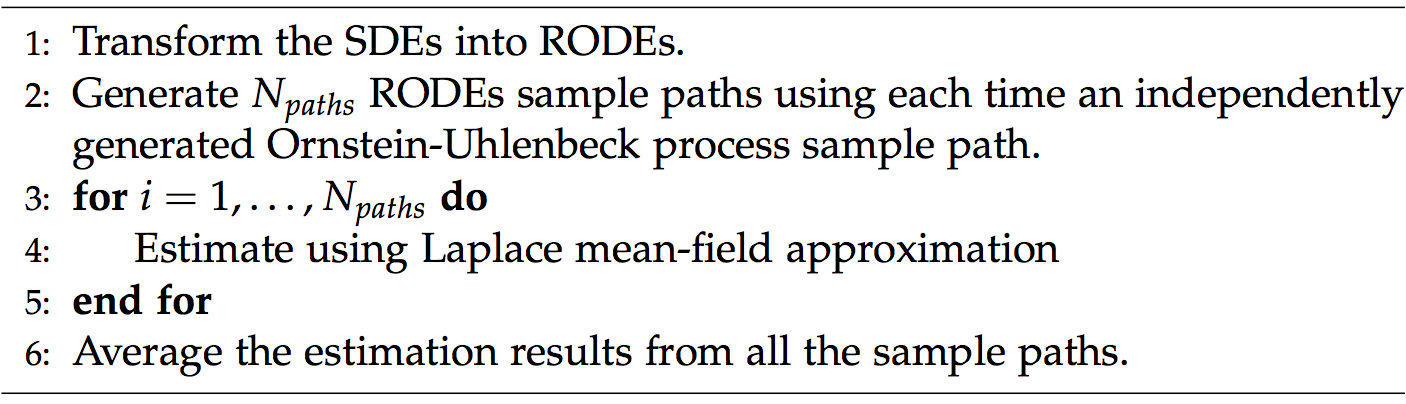
\includegraphics[width=0.9\textwidth]{graphics/lpmf-sde-algorithm}                    
    \end{figure}            
\end{frame}